Die hier vorgestellte Software wird eine große Menge von Schüler- und Moduldaten verarbeiten, die in strukturierten und effizienten Tabellen in einer relationalen
Datenbank gespeichert werden. Dieses RDBMS (Relationale Datenbank Management System) wird eine Schnittstelle zwischen Nutzern und Anwendungen bilden, die für Verwaltungs-,
Zugangs- und Performancefunktionen anbietet. In den folgenden Unterabschnitten werden die gängigsten Datenbanken vorgestellt und anhand ihrer Hauptmerkmale die Datenbanken ermittelt,
die den Anforderungen des Projekts am besten entsprechen. Die Unterschiede zwischen den drei führenden Datenbanken sind nicht so ausgeprägt, so dass der Vergleich zwischen
der beliebtesten und der mäßig bekannten Software erfolgt.Die Auswahl basierte auf den Kriterien von DB-Engines.com für das Ranking der Datenbanken,
d. h. auf der Anzahl der Erwähnungen auf Websites, dem durchschnittlichen Interesse an dem System, der Häufigkeit von Fachdiskussionen über das System, Stellenanzeigen,
die das System erfordern, und der Relevanz in sozialen Medien. Siehe Abbildung \ref{db_engines_ranking}
\begin{figure}[h]
    \begin{center}
        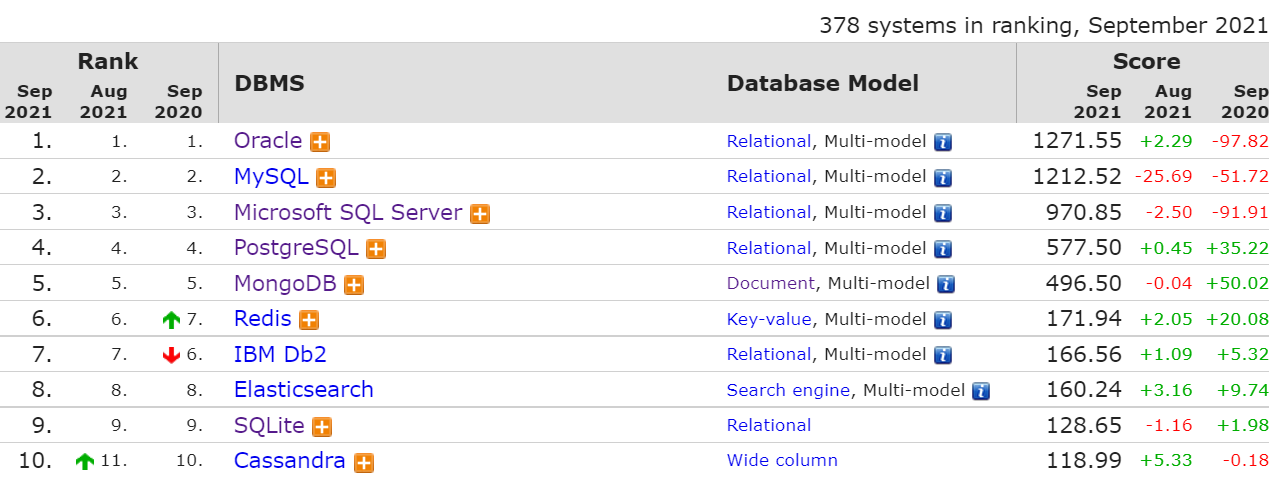
\includegraphics[scale=0.5]{./pics/db_engines_ranking.png}
        \caption{Db-Engines Ranking}
        \label{db_engines_ranking}
    \end{center}
\end{figure}
\newpage